% ------------------------------------------------------------------------------
% TYPO3 CMS 6.2 LTS - What's New - Chapter "Backend Changes" (Spanish Version)
%
% @author	Sergio Catalá <sergio.catala@e-net.info>
% @author	Michel Mix <mmix@autistici.org>
% @license	Creative Commons BY-NC-SA 3.0
% @link		http://typo3.org/download/release-notes/whats-new/
% @language	Spanish
% ------------------------------------------------------------------------------
% Chapter: Backend Changes
% ------------------------------------------------------------------------------

\section{Cambios en Backend}
\begin{frame}[fragile]
	\frametitle{Cambios en Backend}

	\begin{center}\huge{Capítulo 3:}\end{center}
	\begin{center}\huge{\color{typo3darkgrey}\textbf{Cambios en Backend}}\end{center}

\end{frame}

% ------------------------------------------------------------------------------
% Autofocus
% ------------------------------------------------------------------------------
% http://forge.typo3.org/issues/49228

\begin{frame}[fragile]
	\frametitle{Cambios en Backend}
	\framesubtitle{Autenticación en Backend}

 	\begin{itemize}
		\item Autofoco en campo de usuario en el formulario de autenticación del backend (atributo HTML5: \texttt{autofocus="autofocus"})
	\end{itemize}

	\begin{figure}
		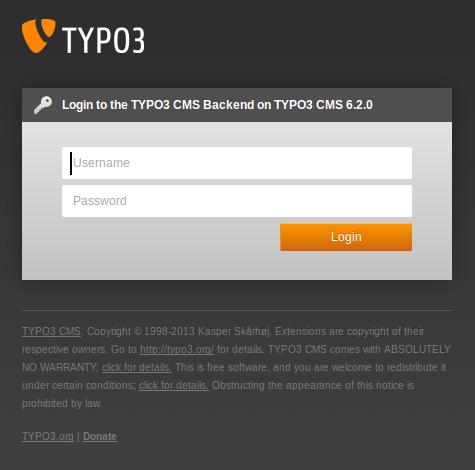
\includegraphics[width=0.4\linewidth]{Images/BackendChanges/BackendLogin.png}
	\end{figure}

\end{frame}

% ------------------------------------------------------------------------------
% Visual Appearance
% ------------------------------------------------------------------------------
% http://forge.typo3.org/issues/48376

\begin{frame}[fragile]
	\frametitle{Cambios en Backend}
	\framesubtitle{Apariencia Visual (1)}

	\begin{columns}[T]

		\begin{column}{.5\textwidth}
			\begin{itemize}
				\item Usabilidad mejorada al hacer correr el diseño
				\item Márgenes entre items de un módulo (columna a la izquierda) incrementados
				\item Basado en un grid de 12px, lo cual ha sido doblado
			\end{itemize}

			\advance\leftskip+2.8cm

			\smaller
				Izquierda: TYPO3 4.5\newline
				Derecha: TYPO3 6.2
			\normalsize
		\end{column}

		\begin{column}{.5\textwidth}
			\begin{figure}\vspace*{-0.4cm}
				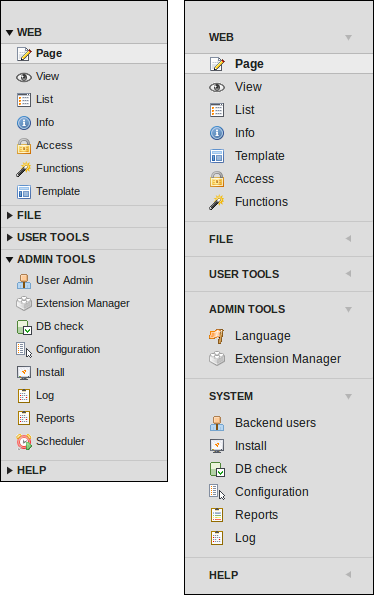
\includegraphics[width=0.6\linewidth]{Images/BackendChanges/VisualAppearance.png}
			\end{figure}
		\end{column}

	\end{columns}

\end{frame}

% ------------------------------------------------------------------------------
% Visual Appearance
% ------------------------------------------------------------------------------

\begin{frame}[fragile]
	\frametitle{Cambios en Backend}
	\framesubtitle{Apariencia Visual (2)}

	\begin{columns}[T]

		\begin{column}{.5\textwidth}

			\begin{itemize}
				\item Módulos de la columna izquierda reestructurados
				\item Módulo "ADMINTOOLS" dividido en dos partes:

					\begin{itemize}
						\item \textbf{ADMINTOOLS} ("Lenguajes" y "Gestor de Extensiones")
						\item \textbf{SYSTEM} (herramientas de bajo nivel, que no muestran la columna del árbol de páginas)
					\end{itemize}

				\item Módulo "TypoScript-Help" eliminado (obsoleto)

			\end{itemize}

		\end{column}

		\begin{column}{.5\textwidth}
			\begin{figure}\vspace*{-0.4cm}
				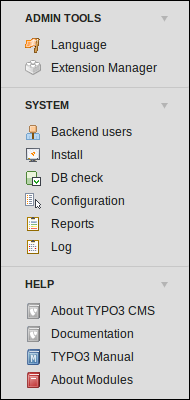
\includegraphics[width=0.35\linewidth]{Images/BackendChanges/AdminTools.png}
			\end{figure}
		\end{column}

	\end{columns}

\end{frame}

% ------------------------------------------------------------------------------
% Visual Appearance
% ------------------------------------------------------------------------------
% http://forge.typo3.org/issues/36017

\begin{frame}[fragile]
	\frametitle{Cambios en Backend}
	\framesubtitle{Apariencia Visual (3)}

	\begin{itemize}
		\item \texttt{<h1>}-cabeceras en área principal usan fuente TYPO3 "Share" consistentemente
	\end{itemize}

	\begin{figure}
		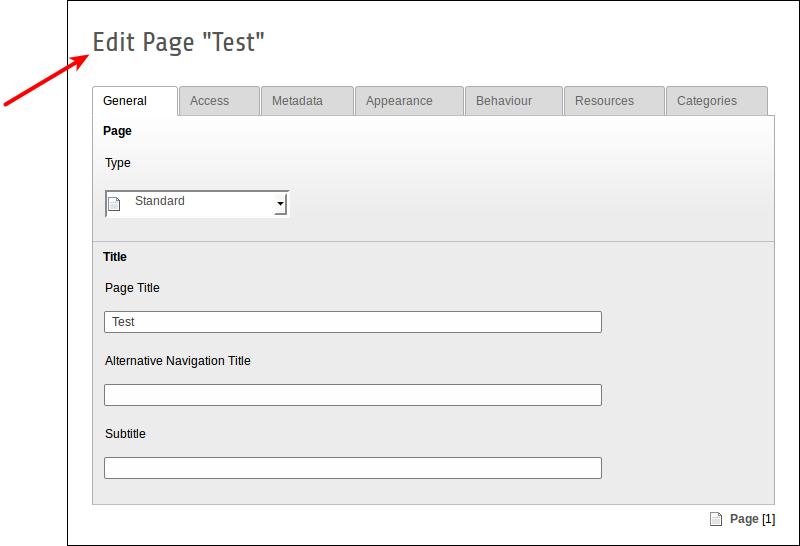
\includegraphics[width=0.6\linewidth]{Images/BackendChanges/ConsistantFont.png}
	\end{figure}

\end{frame}

% ------------------------------------------------------------------------------
% Visual Appearance
% ------------------------------------------------------------------------------
% http://forge.typo3.org/issues/41631

\begin{frame}[fragile]
	\frametitle{Cambios en Backend}
	\framesubtitle{Apariencia Visual (4)}

	\begin{itemize}
		\item Módulo "Informes" muestra nuevo icono
	\end{itemize}

	\begin{figure}
		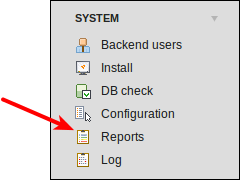
\includegraphics[width=0.35\linewidth]{Images/BackendChanges/ModuleReportsIcon.png}
	\end{figure}

\end{frame}

% ------------------------------------------------------------------------------
% Filelist: Drag&Drop File Upload
% ------------------------------------------------------------------------------
% http://forge.typo3.org/issues/47005

\begin{frame}[fragile]
	\frametitle{Cambios en Backend}
	\framesubtitle{Subida de Ficheros Arrastrar y Soltar (1)}

	\begin{itemize}
		\item Funcionalidad HTML5 de subida de ficheros Arrastrar y Soltar implementada en la lista de ficheros

	\end{itemize}

	\begin{figure}
		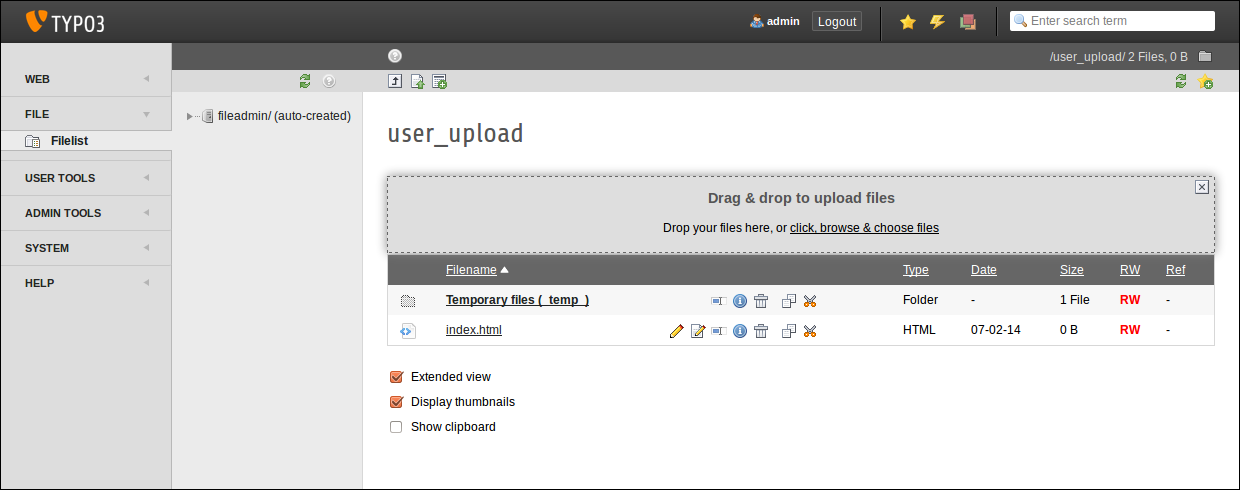
\includegraphics[width=0.95\linewidth]{Images/BackendChanges/DragDropFileUpload.png}
	\end{figure}

\end{frame}

% ------------------------------------------------------------------------------
% Drag&Drop File Upload Via Content Elements
% (slide added in March 2014)
% ------------------------------------------------------------------------------

\begin{frame}[fragile]
	\frametitle{Cambios en Backend}
	\framesubtitle{Subida de Ficheros Arrastrar y Soltar (2)}

	\begin{itemize}
		\item ... y vía elementos de contenido (botón: "Seleccionar y subir ficheros")

	\end{itemize}

	\begin{figure}
		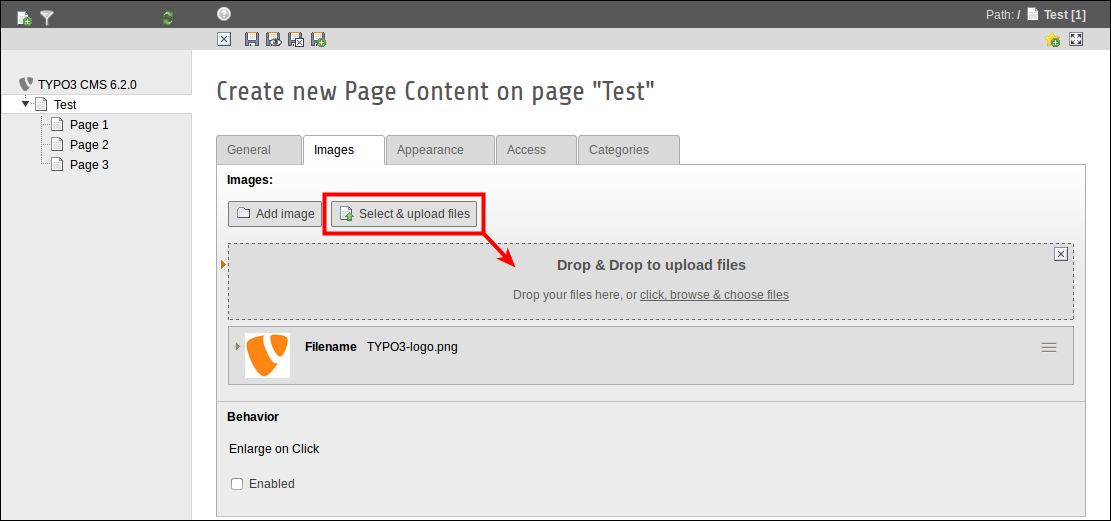
\includegraphics[width=0.95\linewidth]{Images/BackendChanges/SelectAndUploadFiles.png}
	\end{figure}

\end{frame}

% ------------------------------------------------------------------------------
% Backend Users
% ------------------------------------------------------------------------------
% http://forge.typo3.org/issues/43053

\begin{frame}[fragile]
	\frametitle{Cambios en Backend}
	\framesubtitle{Usabilidad: Usuarios del Backend}

	\begin{itemize}
		\item Se muestra nombre de usuario y nombre real\newline
		(primera columna en la vista de lista)
		\item Clic en los enlaces de nombre (de usuario) para\newline
		editar registro de usuario
		\item Botón de borrado añadido a la vista de lista

	\end{itemize}

	\begin{figure}
		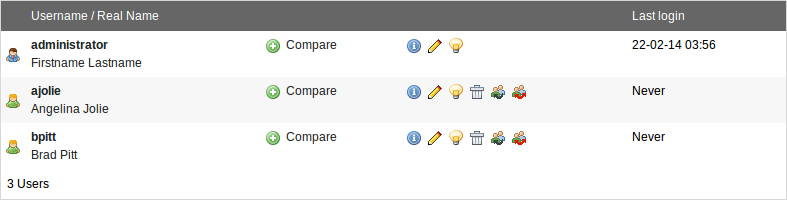
\includegraphics[width=0.95\linewidth]{Images/BackendChanges/BackendUserList.png}
	\end{figure}

\end{frame}

% ------------------------------------------------------------------------------
% Live Search
% ------------------------------------------------------------------------------
% http://forge.typo3.org/issues/35358

\begin{frame}[fragile]
	\frametitle{Cambios en Backend}
	\framesubtitle{Búsqueda en Vivo (1)}

	\begin{itemize}
		\item Tooltip muestra tanto el UID como el PID en "búsqueda en tiempo real"
		\item Cuando, tras una búsqueda, se cierra otra vez el formulario de edición, se muestra la vista de lista de la página (no una página vacía)
	\end{itemize}

	\begin{figure}
		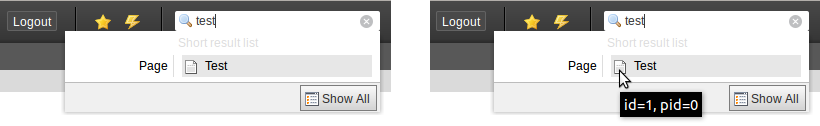
\includegraphics[width=0.8\linewidth]{Images/BackendChanges/LiveSearchTooltip.png}
	\end{figure}

\end{frame}

% ------------------------------------------------------------------------------
% Live Search
% ------------------------------------------------------------------------------

\begin{frame}[fragile]
	\frametitle{Cambios en Backend}
	\framesubtitle{Búsqueda en Vivo (2)}

	\begin{itemize}
		\item En TYPO3 < 6.2, para las páginas, sólo se tienen en cuenta los campos \texttt{title} y \texttt{uid} de la base de datos
		\item En TYPO3 >= 6.2, puede añadirse el campo \texttt{alias} a la búsqueda\newline
			(requiere UserTSconfig: \texttt{options.pageTree.searchInAlias = 1})
	\end{itemize}

	\begin{figure}
		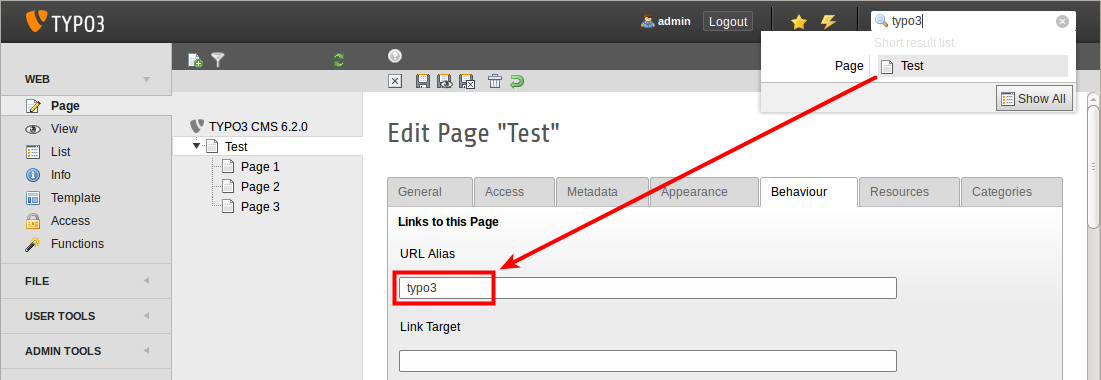
\includegraphics[width=0.95\linewidth]{Images/BackendChanges/LiveSearchInAlias.png}
	\end{figure}

\end{frame}

% ------------------------------------------------------------------------------
% File Abstraction Layer
% ------------------------------------------------------------------------------

\begin{frame}[fragile]
	\frametitle{Cambios en Backend}
	\framesubtitle{Capa de Abstracción de Ficheros}

	\begin{itemize}
		\item Se muestra el nombre del fichero y el título en la cabecera del elemento FAL
	\end{itemize}

	\begin{figure}
		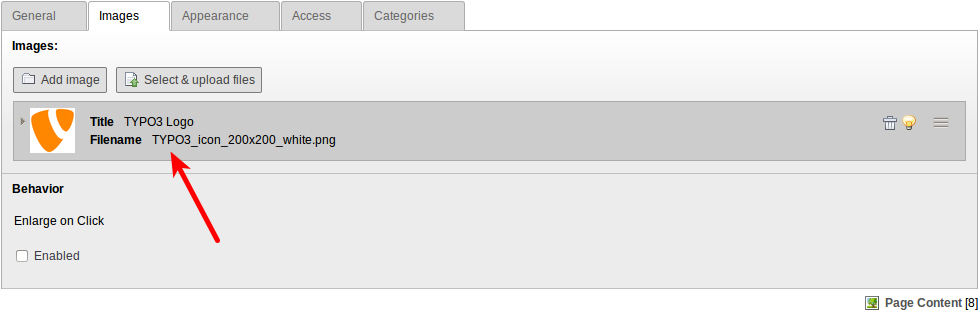
\includegraphics[width=0.95\linewidth]{Images/BackendChanges/FalTitleAndFilename.png}
	\end{figure}

\end{frame}

% ------------------------------------------------------------------------------
% File Abstraction Layer
% ------------------------------------------------------------------------------

\begin{frame}[fragile]
	\frametitle{Cambios en Backend}
	\framesubtitle{Capa de Abstracción de Ficheros (EXT:filemetadata) (1)}

	\begin{itemize}
		\item Extensión del sistema "filemetadata" añade tabs para mostrar meta datos\newline
			\small(la extensión viene con el núcleo, pero no se instala por defecto)\normalsize
	\end{itemize}

	\begin{figure}
		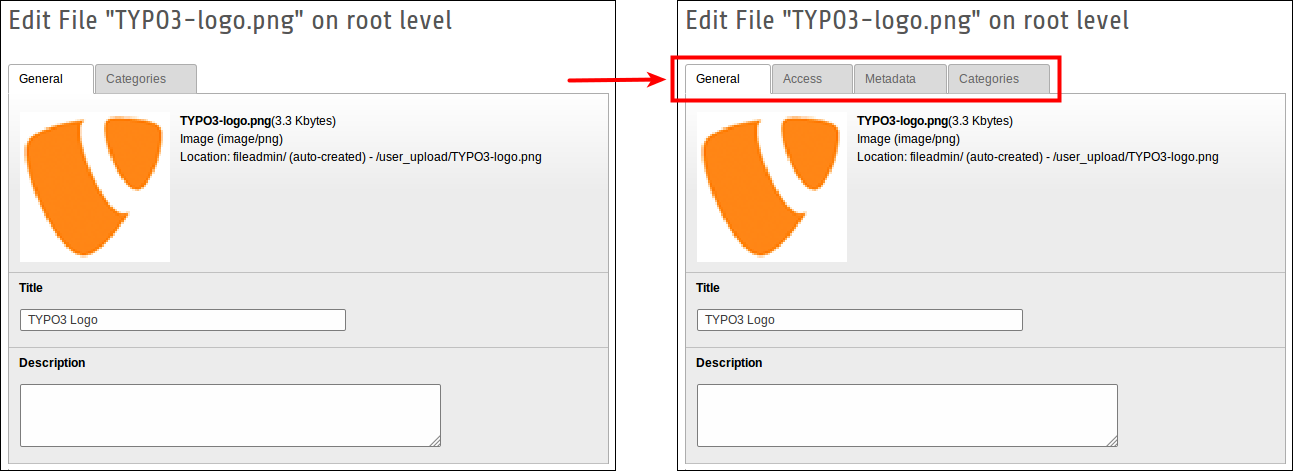
\includegraphics[width=0.95\linewidth]{Images/BackendChanges/FileMetaDataTabs.png}
	\end{figure}
\end{frame}

% ------------------------------------------------------------------------------
% File Abstraction Layer
% ------------------------------------------------------------------------------

\begin{frame}[fragile]
	\frametitle{Cambios en Backend}
    	\framesubtitle{Capa de Abstracción de Ficheros (EXT:filemetadata) (2)}

	\begin{figure}
		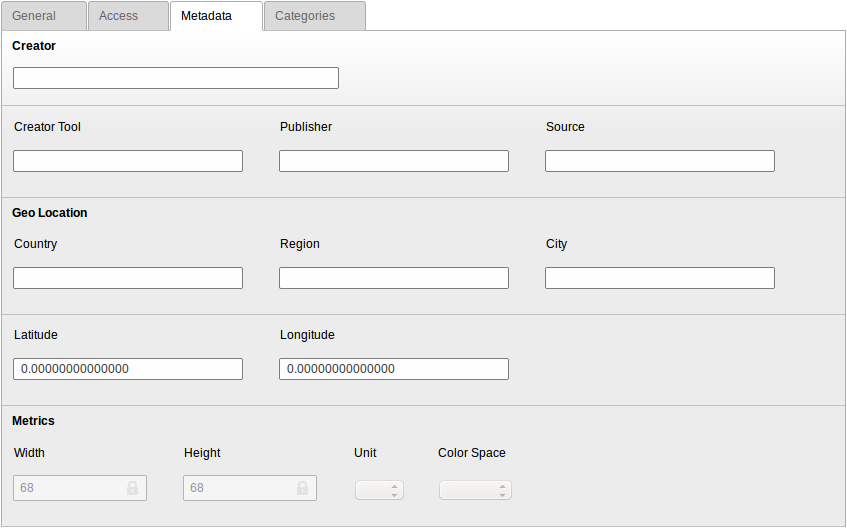
\includegraphics[width=0.8\linewidth]{Images/BackendChanges/FileMetaData.png}
	\end{figure}

\end{frame}

% ------------------------------------------------------------------------------
% File Abstraction Layer
% ------------------------------------------------------------------------------

\begin{frame}[fragile]
	\frametitle{Cambios en Backend}
	\framesubtitle{Capa de Abstracción de Ficheros}

	\begin{itemize}
		\item Ahora es posible traducir meta datos FAL en lenguajes del frontend
	\end{itemize}

	\begin{figure}
		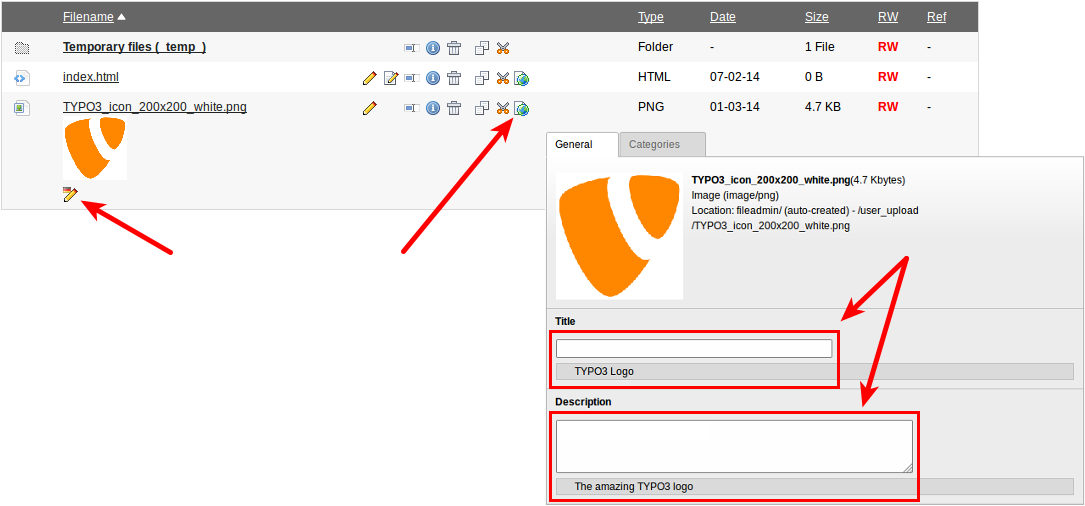
\includegraphics[width=0.95\linewidth]{Images/BackendChanges/FalTranslateMetaData.png}
	\end{figure}

\end{frame}

% ------------------------------------------------------------------------------
% Module: Documentation
% ------------------------------------------------------------------------------

\begin{frame}[fragile]
	\frametitle{Cambios en Backend}
	\framesubtitle{Módulo: Documentación (1)}

	\begin{columns}[T]

		\begin{column}{.5\textwidth}
			\begin{itemize}
				\item Módulo "Documentación" permite a los usuarios BE descargar y ver manuales
				\item Nuevas instalaciones TYPO3 cargan este módulo por defecto
				\item Función "Descargar Documentación" descarga manuales (ver ilustración)
			\end{itemize}
		\end{column}

		\begin{column}{.5\textwidth}
			\begin{figure}\vspace*{-0.4cm}
				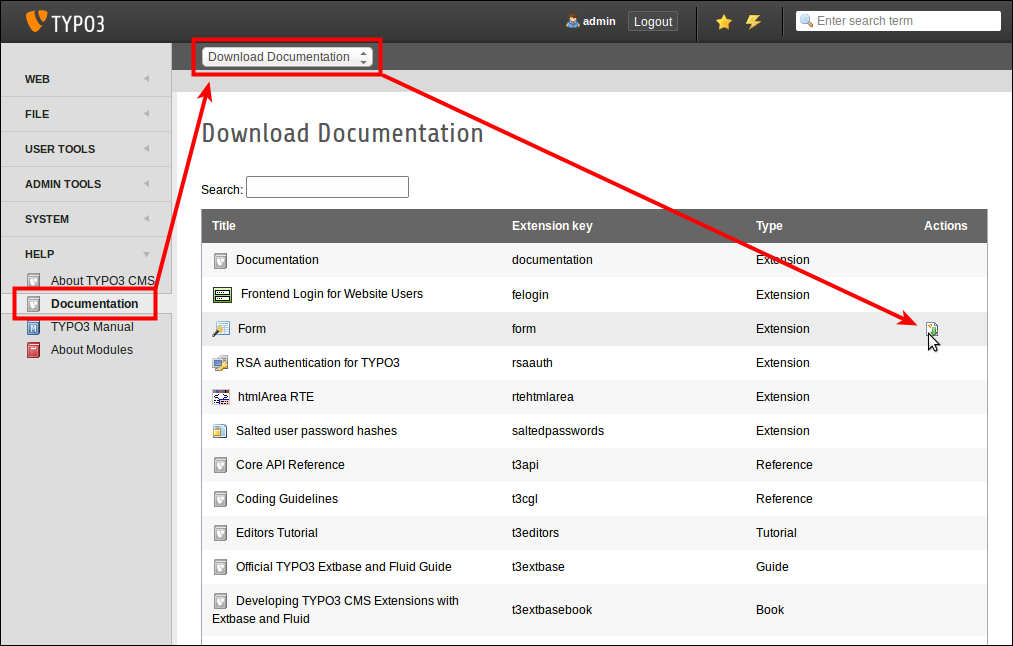
\includegraphics[width=1\linewidth]{Images/BackendChanges/DownloadDocumentation.png}
			\end{figure}
		\end{column}

	\end{columns}

\end{frame}

% ------------------------------------------------------------------------------
% Module: Documentation
% ------------------------------------------------------------------------------

\begin{frame}[fragile]
	\frametitle{Cambios en Backend}
	\framesubtitle{Módulo: Documentación (2)}

	\begin{itemize}
		\item Se usa el Gestor de Extensiones para cargar "Documentación" en una instalación TYPO3 actualizada
		\item Función "Mostrar Documentación" muestra manuales descargados
	\end{itemize}

	\begin{figure}
		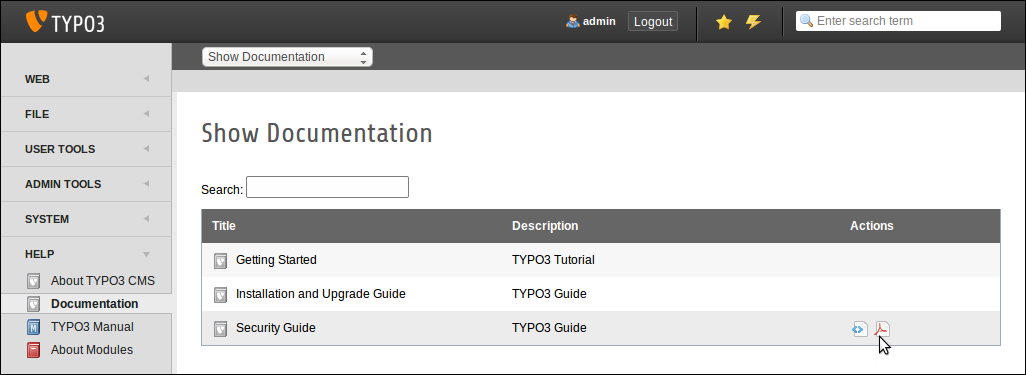
\includegraphics[width=0.95\linewidth]{Images/BackendChanges/ShowDocumentation.png}
	\end{figure}

\end{frame}

% ------------------------------------------------------------------------------
% Removed: TypoScript Help
% ------------------------------------------------------------------------------
% http://forge.typo3.org/issues/47931

\begin{frame}[fragile]
	\frametitle{Cambios en Backend}
	\framesubtitle{Eliminada: Ayuda TypoScript}

 	\begin{itemize}
		\item EXT:tsconfig\_help ("Referencia Rápida TSconfig") eliminada\newline
			\small(información anticuada y no mantenida desde TYPO3 CMS 4.1)
	\end{itemize}

	\begin{figure}
		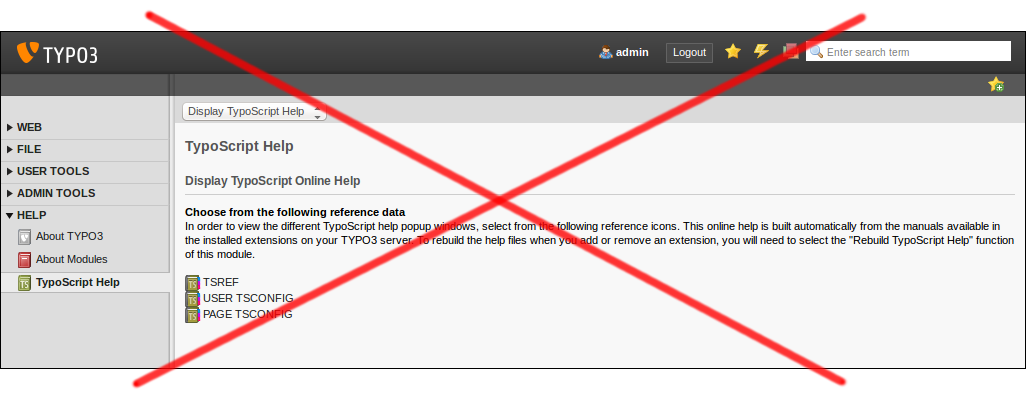
\includegraphics[width=0.95\linewidth]{Images/BackendChanges/TypoScriptHelpRemovedCrossed.png}
	\end{figure}

\end{frame}


% ------------------------------------------------------------------------------
% Scheduler
% ------------------------------------------------------------------------------

\begin{frame}[fragile]
	\frametitle{Cambios en Backend}
	\framesubtitle{Programador (1)}

	\begin{itemize}
		\item Se puede borrar tarea del programador en vista de edición\newline
			\small(en TYPO3 < 6.2, función de borrado estaba disponible sólo en vista de lista)\normalsize
	\end{itemize}

	\begin{figure}
		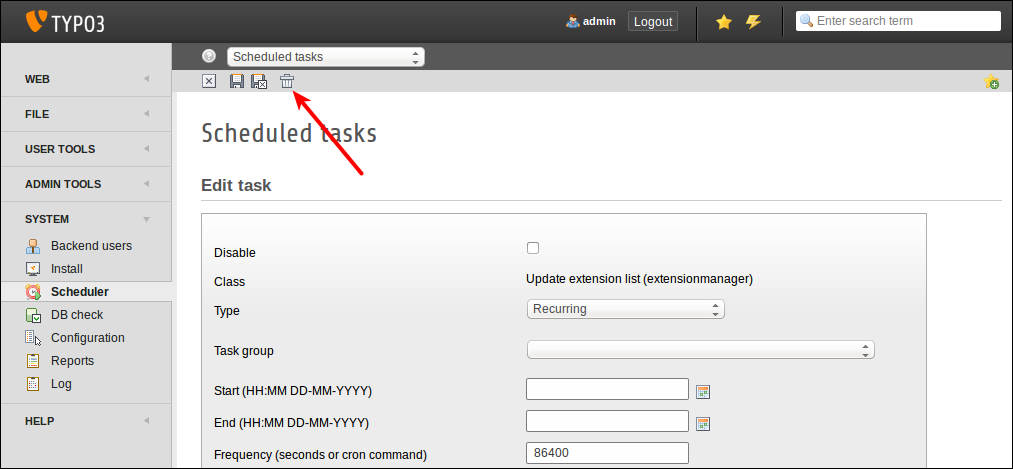
\includegraphics[width=0.95\linewidth]{Images/BackendChanges/DeleteSchedulerTaskInEditView.png}
	\end{figure}

\end{frame}

% ------------------------------------------------------------------------------
% Scheduler
% ------------------------------------------------------------------------------

\begin{frame}[fragile]
	\frametitle{Cambios en Backend}
	\framesubtitle{Programador (2)}

	\begin{itemize}
		\item Puede asignarse una descripción a las tareas del programador y que se muestren como cabeceras en la vista de lista, o como tooltips (ver próxima diapositiva)
	\end{itemize}

	\begin{figure}
		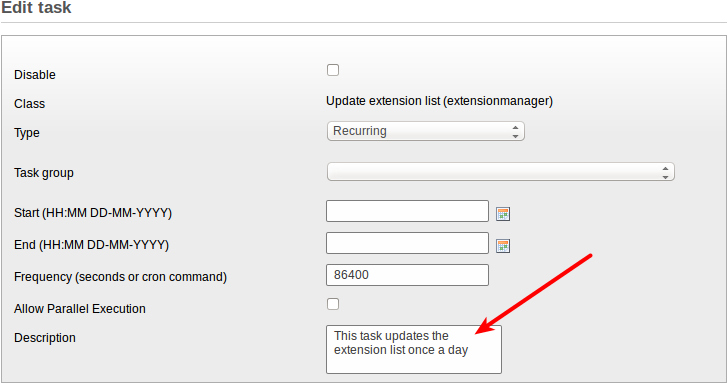
\includegraphics[width=0.7\linewidth]{Images/BackendChanges/SchedulerTaskDescription.png}
	\end{figure}

\end{frame}

% ------------------------------------------------------------------------------
% Scheduler
% ------------------------------------------------------------------------------

\begin{frame}[fragile]
	\frametitle{Cambios en Backend}
	\framesubtitle{Programador (3)}

	\begin{itemize}
		\item Descripción de la tarea como subcabecera\newline
			\small(esta característica necesita activarse en la configuración de la extensión)\normalsize
	\end{itemize}

	\begin{figure}
		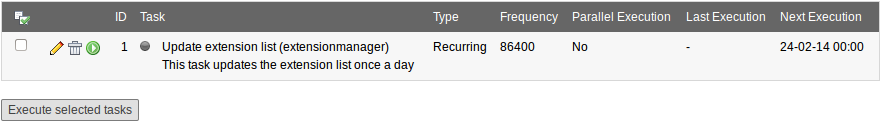
\includegraphics[width=0.95\linewidth]{Images/BackendChanges/SchedulerTaskDescriptionAsSubheader.png}
	\end{figure}

	\begin{itemize}
		\item Descripción de la tarea como tooltip ("hover")
	\end{itemize}

	\begin{figure}
		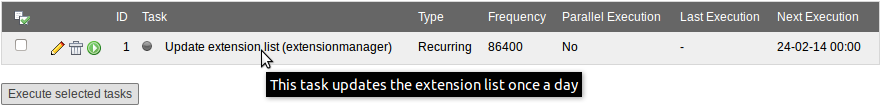
\includegraphics[width=0.95\linewidth]{Images/BackendChanges/SchedulerTaskDescriptionAsTooltip.png}
	\end{figure}

\end{frame}

% ------------------------------------------------------------------------------
% Scheduler
% ------------------------------------------------------------------------------

\begin{frame}[fragile]
	\frametitle{Cambios en Backend}
    	\framesubtitle{Programador (4)}

	\begin{itemize}
		\item Ahora es posible agrupar tareas del programador
		\item Añadir registros "grupo de tareas del programador" a la página raíz (UID: 0)
	\end{itemize}

	\begin{figure}
		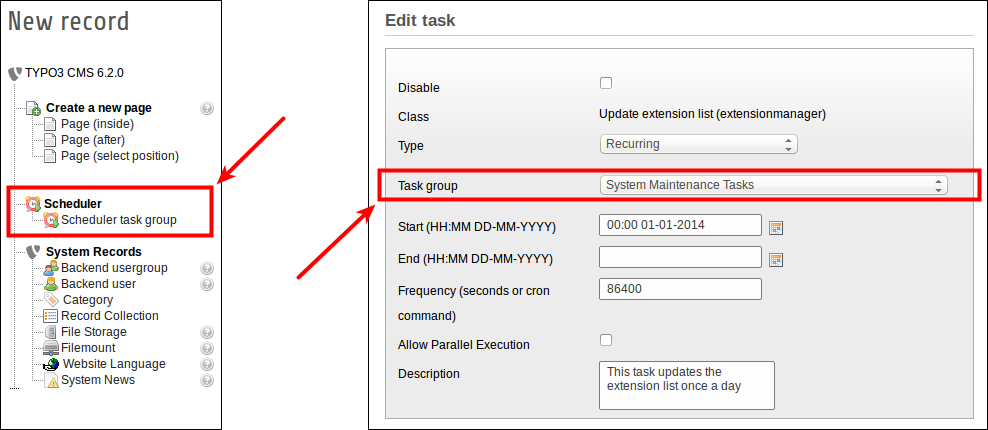
\includegraphics[width=0.85\linewidth]{Images/BackendChanges/SchedulerTaskGroup.png}
	\end{figure}

\end{frame}

% ------------------------------------------------------------------------------
% System Extension: Form
% ------------------------------------------------------------------------------
% http://forge.typo3.org/issues/38094

\begin{frame}[fragile]
	\frametitle{Cambios en Backend}
	\framesubtitle{Extensión del Sistema: Form}

	\begin{columns}[T]

		\begin{column}{.5\textwidth}
			\begin{itemize}
				\item Nuevo post-procesador para cObject FORM: \textbf{redirect}\newline
					(redireccionar tras envío del formulario)
				\item Se analiza el valor por \texttt{typolink} (función TypoScript),\newline
					lo que significa que el valor puede ser un ID de página o una URL
			\end{itemize}
		\end{column}

		\begin{column}{.5\textwidth}
			\begin{figure}\vspace*{-0.4cm}
				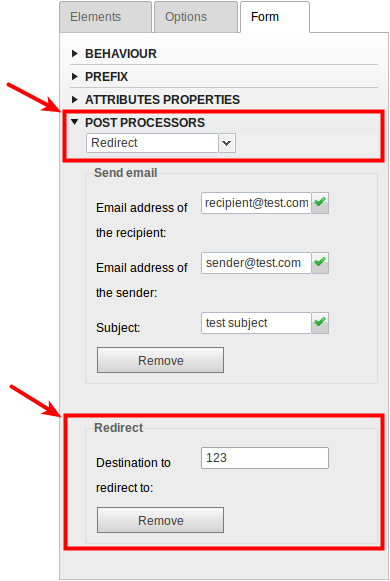
\includegraphics[width=0.65\linewidth]{Images/BackendChanges/FormRedirectPostProcessor.png}
			\end{figure}
		\end{column}
	\end{columns}
\end{frame}

% ------------------------------------------------------------------------------
% Module: List
% ------------------------------------------------------------------------------
% http://forge.typo3.org/issues/49810

\begin{frame}[fragile]
	\frametitle{Cambios en Backend}
	\framesubtitle{Módulo Lista}

	\begin{itemize}
		\item Columnas adicionales "UID" y "PID" en vista de lista para no-administradores
	\end{itemize}

	\begin{figure}
		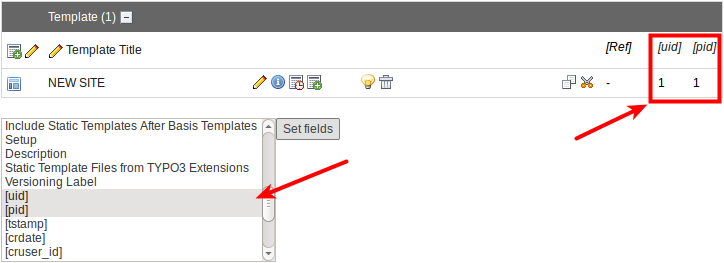
\includegraphics[width=0.95\linewidth]{Images/BackendChanges/AdditionalColumnsInListModule.png}
	\end{figure}

\end{frame}

% ------------------------------------------------------------------------------
% File Abstraction Layer
% ------------------------------------------------------------------------------
% http://forge.typo3.org/issues/50827
% http://forge.typo3.org/issues/51097

\begin{frame}[fragile]
	\frametitle{Cambios en Backend}
	\framesubtitle{Capa de Abstracción de Ficheros}

	\begin{itemize}
		\item Si el indexador detecta un fichero que falta, se muestra un mensaje y se fija un flag en el registro de la base de datos
		\item Módulo "Informes" lista también esto como un asunto
		\item Cuando el fichero reaparece, se resetean el mensaje y el flag
	\end{itemize}

	\begin{columns}[T]

		\begin{column}{.5\textwidth}
			\begin{figure}
				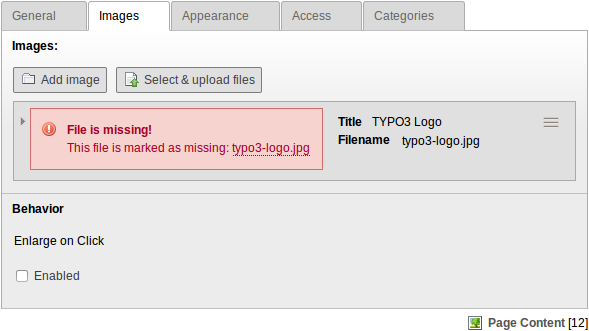
\includegraphics[width=0.95\linewidth]{Images/BackendChanges/FalMissingFileContentElement.png}
			\end{figure}
		\end{column}

		\begin{column}{.5\textwidth}
			\begin{figure}
				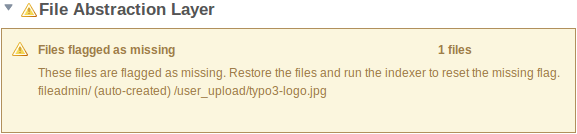
\includegraphics[width=0.95\linewidth]{Images/BackendChanges/FalMissingFileReportsModule.png}
			\end{figure}
		\end{column}

	\end{columns}

\end{frame}

% ------------------------------------------------------------------------------
% Menu/Sitemap: Categories-based Menus
% ------------------------------------------------------------------------------
% http://forge.typo3.org/issues/51161

\begin{frame}[fragile]
	\frametitle{Cambios en Backend}
	\framesubtitle{Menús basados en Categorías (1)}

	\begin{itemize}
		\item Elemento de contenido "Menú/Mapa del sitio" puede crear un menú, basado en categorías
	\end{itemize}

	\begin{figure}
		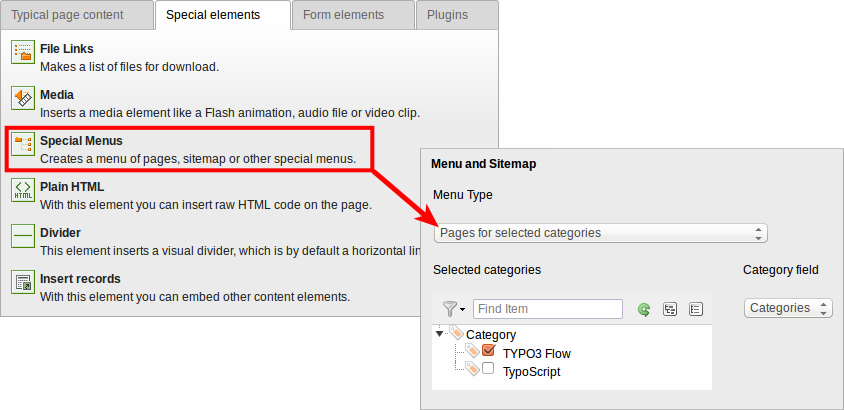
\includegraphics[width=0.8\linewidth]{Images/BackendChanges/CategoryBasedMenus.png}
	\end{figure}

\end{frame}

% ------------------------------------------------------------------------------
% Menu/Sitemap: Category-based Menus
% (slide added in March 2014)
% ------------------------------------------------------------------------------

\begin{frame}[fragile]
	\frametitle{Cambios en Backend}
	\framesubtitle{Menús basados en Categorías (2)}

	\begin{itemize}
		\item Otro nuevo tipo de menú: "\underline{Elementos de contenido} para las categorías seleccionadas"
	\end{itemize}

	\begin{figure}
		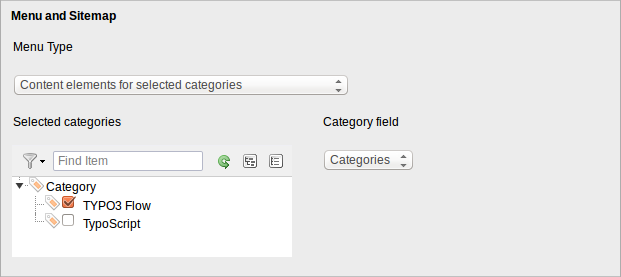
\includegraphics[width=0.6\linewidth]{Images/BackendChanges/ContentElementsForSelectedCategories.png}
	\end{figure}

\end{frame}

% ------------------------------------------------------------------------------
% Sorting Categories
% ------------------------------------------------------------------------------
% http://forge.typo3.org/issues/51590

\begin{frame}[fragile]
	\frametitle{Cambios en Backend}
	\framesubtitle{Ordenando Categorías}

 	\begin{itemize}
		\item Ahora pueden ordenarse las categorías\newline
			\small(en TYPO3 < 6.2, las categorías siempre se ordenan alfabéticamente)\normalsize
	\end{itemize}

	\begin{figure}
		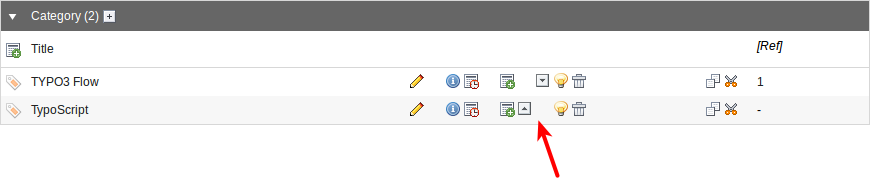
\includegraphics[width=0.95\linewidth]{Images/BackendChanges/CategorySorting.png}
	\end{figure}

\end{frame}

% ------------------------------------------------------------------------------
% Category Visibility
% ------------------------------------------------------------------------------
% http://forge.typo3.org/issues/52718

\begin{frame}[fragile]
	\frametitle{Cambios en Backend}
	\framesubtitle{Visibilidad de Categoría}

 	\begin{itemize}
		\item Puede restringirse la visibilidad de categorías para usuarios/grupos BE
	\end{itemize}

	\begin{figure}
		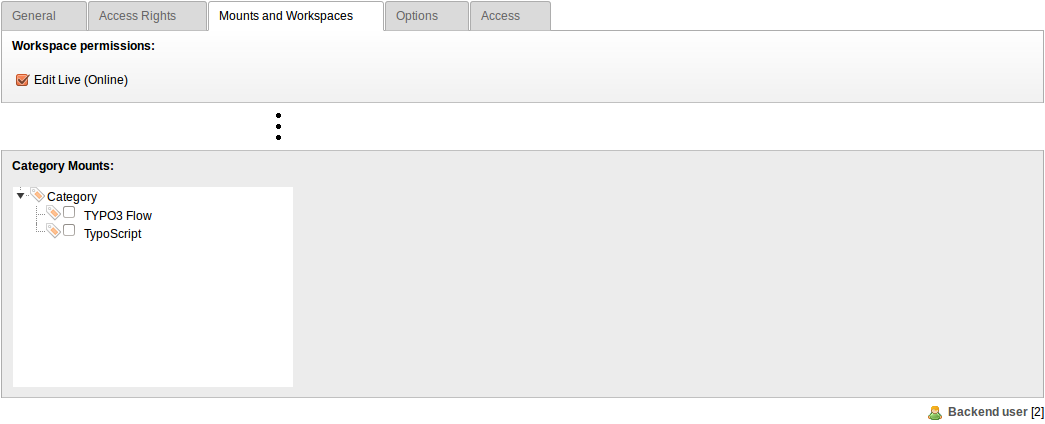
\includegraphics[width=0.95\linewidth]{Images/BackendChanges/CategoryVisibility.png}
	\end{figure}

\end{frame}

% ------------------------------------------------------------------------------
% "New Content" icon always visible
% ------------------------------------------------------------------------------
% http://forge.typo3.org/issues/48938
% http://forge.typo3.org/issues/51480

\begin{frame}[fragile]
	\frametitle{Cambios en Backend}
	\framesubtitle{Usabilidad}

 	\begin{itemize}
		\item Icono "nuevo contenido" está siempre visible si la columna está vacía\newline
			\small(esto ayuda a los editores a entender qué pueden hacer)\normalsize
	\end{itemize}

	\begin{figure}
		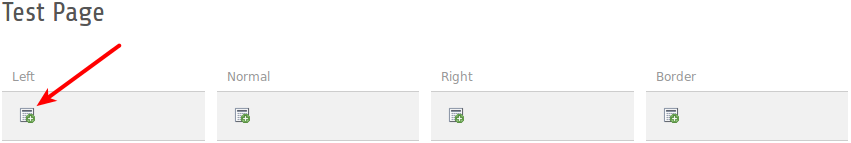
\includegraphics[width=0.95\linewidth]{Images/BackendChanges/NewContentIconAlwaysVisible.png}
	\end{figure}

\end{frame}

% ------------------------------------------------------------------------------
% Module "Functions": Hide In Menus
% ------------------------------------------------------------------------------
% http://forge.typo3.org/issues/51017

\begin{frame}[fragile]
	\frametitle{Cambios en Backend}
	\framesubtitle{Funciones}

	\begin{itemize}
		\item Al crear múltiples páginas en el módulo "funciones", un nuevo checkbox permite a los editores esconder estas páginas en los menús
			\small(muy útil, al crear un número de páginas a la vez)\normalsize
	\end{itemize}

	\begin{figure}
		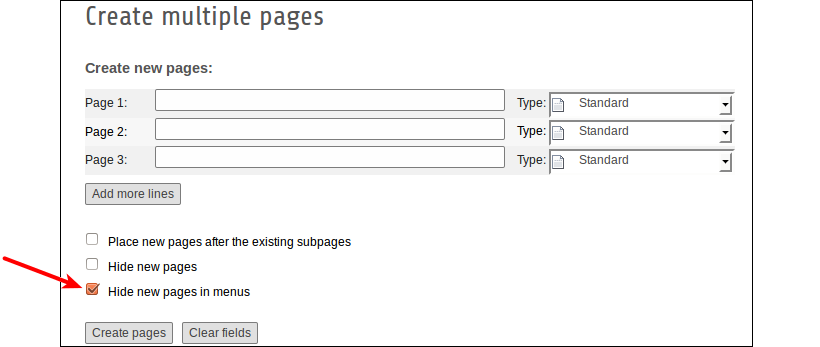
\includegraphics[width=0.85\linewidth]{Images/BackendChanges/CreateMultiplePagesHideInMenu.png}
	\end{figure}

\end{frame}

% ------------------------------------------------------------------------------
% Extension Manager: Upload Extensions
% ------------------------------------------------------------------------------
% http://forge.typo3.org/issues/51776
% http://forge.typo3.org/issues/51437

\begin{frame}[fragile]
	\frametitle{Cambios en Backend}
	\framesubtitle{Gestor de Extensiones}

 	\begin{itemize}
		\item Se puede subir una extensión vía la función "Conseguir Extensiones"
	\end{itemize}

	\begin{figure}
		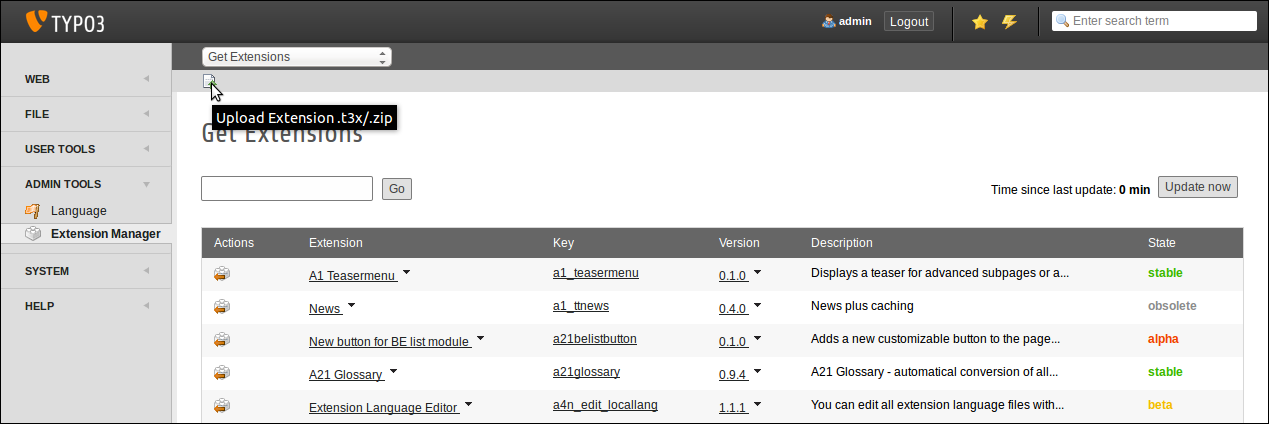
\includegraphics[width=0.95\linewidth]{Images/BackendChanges/UploadExtension.png}
	\end{figure}

\end{frame}

% ------------------------------------------------------------------------------
% Recycler
% ------------------------------------------------------------------------------
% http://forge.typo3.org/issues/52324

\begin{frame}[fragile]
	\frametitle{Cambios en Backend}
	\framesubtitle{Reciclaje}

 	\begin{itemize}
		\item Pueden ordenarse los registros de reciclaje por marca de tiempo\newline
			\small(esto ayuda a los usuarios a decidir si recuperar un registro específico o no)\normalsize
	\end{itemize}

	\begin{figure}
		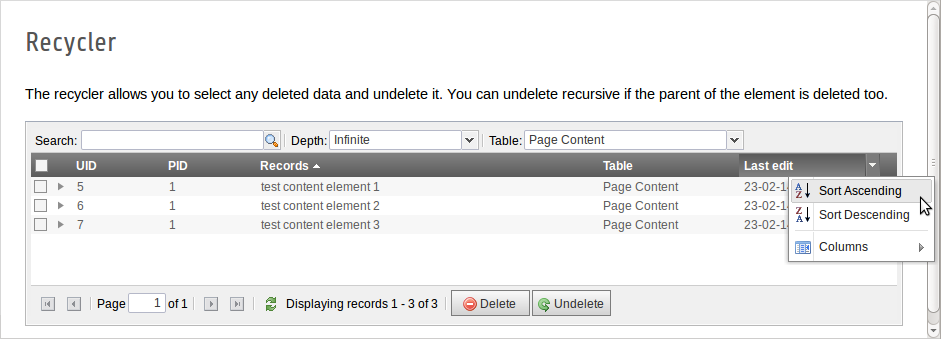
\includegraphics[width=0.95\linewidth]{Images/BackendChanges/RecyclerSortRecord.png}
	\end{figure}

\end{frame}

% ------------------------------------------------------------------------------
% File/Directory Permissions
% ------------------------------------------------------------------------------

\begin{frame}[fragile]
	\frametitle{Cambios en Backend}
	\framesubtitle{Permisos Fichero/Directorio}

 	\begin{itemize}
		\item Permisos de fichero/directorio mucho más granulares para usuarios/grupos BE
			\begingroup\color{typo3red}\textbf{(1)}\endgroup
		\item Esto es posible desde TYPO3 6.0, pero sólo vía UserTSconfig
			\begingroup\color{typo3red}\textbf{(2)}\endgroup
	\end{itemize}

	\begin{figure}
		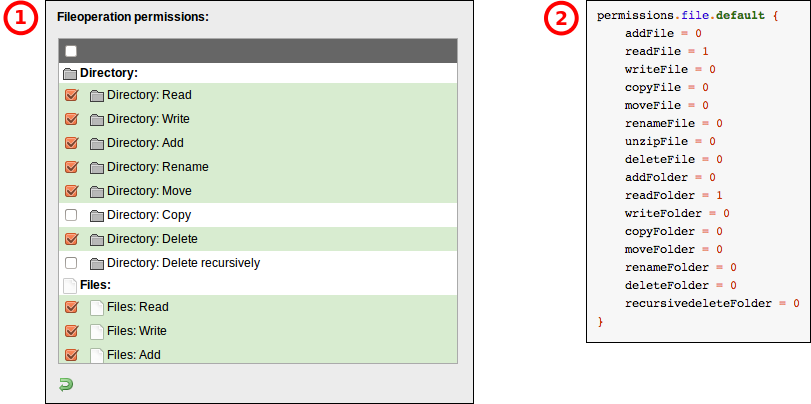
\includegraphics[width=0.75\linewidth]{Images/BackendChanges/FileAndDirectoryPermissions.png}
	\end{figure}

\end{frame}

% ------------------------------------------------------------------------------
% OpenID
% ------------------------------------------------------------------------------

\begin{frame}[fragile]
	\frametitle{Cambios en Backend}
	\framesubtitle{OpenID (1)}

 	\begin{itemize}
		\item Puede configurarse OpenID para la autenticación del usuario BE usando un asistente
		\item Se requiere EXT:openid (extensión del sistema) para esta característica
	\end{itemize}

	\begin{figure}
		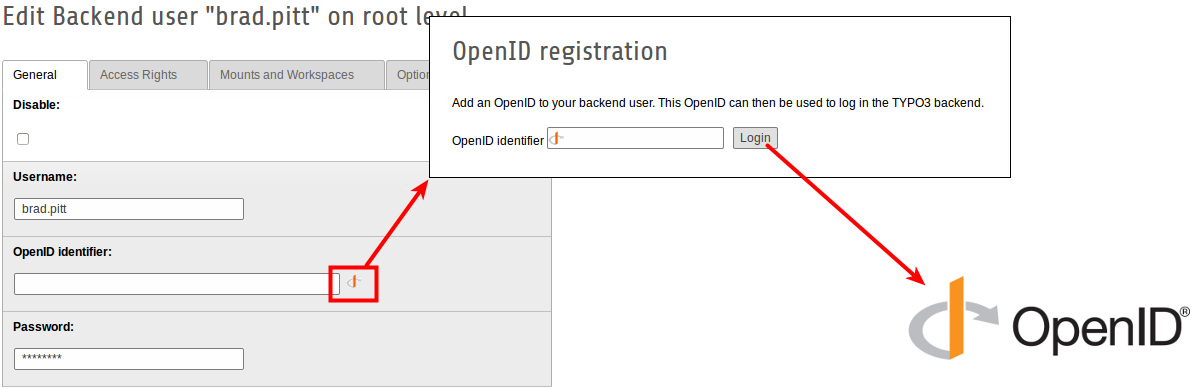
\includegraphics[width=0.95\linewidth]{Images/BackendChanges/OpenIdWizard.png}
	\end{figure}

\end{frame}

% ------------------------------------------------------------------------------
% OpenID
% ------------------------------------------------------------------------------

\begin{frame}[fragile]
	\frametitle{Cambios en Backend}
	\framesubtitle{OpenID (2)}

 	\begin{itemize}
		\item Puede configurarse OpenID para la autenticación del usuario BE usando un asistente
		\item Se requiere EXT:openid (extensión del sistema) para esta característica
	\end{itemize}

	\begin{figure}
		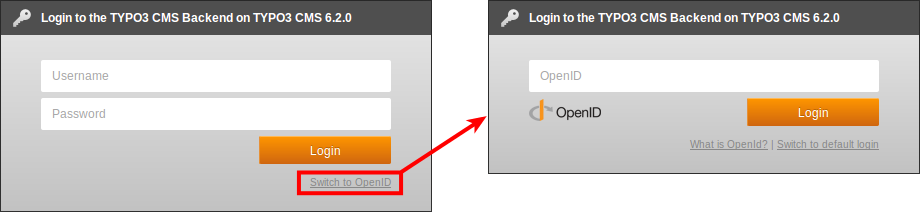
\includegraphics[width=0.8\linewidth]{Images/BackendChanges/OpenIdLogin.png}
	\end{figure}

 	\begin{itemize}
		\item Más detalles sobre OpenID:\newline
			\small\url{http://openid.net}\normalsize
	\end{itemize}

\end{frame}

% ------------------------------------------------------------------------------
% Workspaces
% ------------------------------------------------------------------------------
% http://forge.typo3.org/issues/50223
% http://forge.typo3.org/issues/50224

\begin{frame}[fragile]
	\frametitle{Cambios en Backend}
	\framesubtitle{Áreas de trabajo}

 	\begin{itemize}
		\item Editores/usuarios pueden definir a quién notificar, sin limitar esto a nivel de sistema
		\item Tabulador "Todos" ahora es visible para \underline{todos} los usuarios
	\end{itemize}

	\begin{figure}
		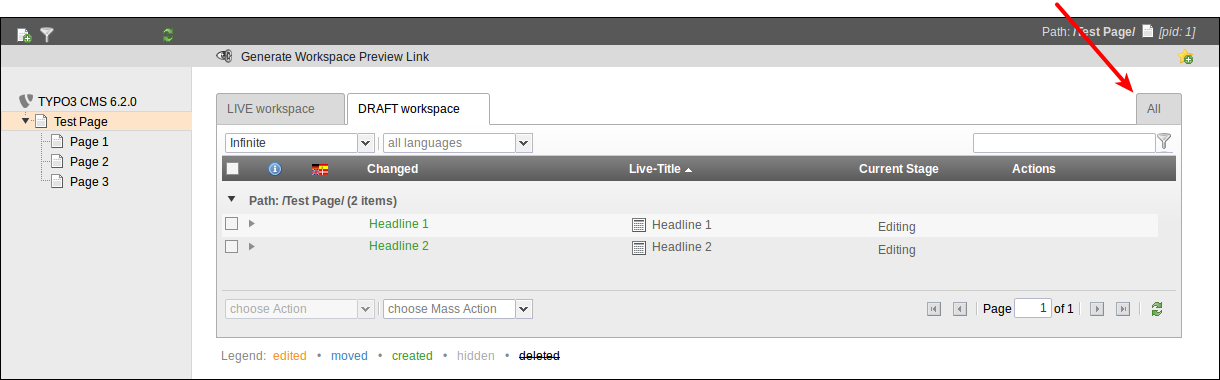
\includegraphics[width=0.95\linewidth]{Images/BackendChanges/WorkspacesTabAll.png}
	\end{figure}

\end{frame}

% ------------------------------------------------------------------------------

